\chapter{Results}

In this chapter the verification and validation of the developed sensor system are described. The verification is a set of tests designed to review whether or not the system meets the requirements specified in the Chapter \ref{obj} Objectives. The validation is done by analyzing the data gathered during a number of experiments in the bioreactor.

\section{Verification}

\subsection{Spacial Resolution}

Requirement: The system shall have a spacial resolution in the order of \unit[10]{mm}.\\

An inspection of the physical size of the sensor and their placement on the array, drawn in Figure \ref{fig:sensarray}, shows us a sensor size of \unit[10x11]{mm} arranged on a grid of \unit[25x50]{mm}. The theoretical minimal grid size achievable with the chosen sensor size and a minimum distance between electrodes of \unit[1]{mm} is \unit[11x12]{mm}.
This grid size is the physical limitation of the spacial resolution and by being well within the order of \unit[10]{mm} meets the requirement.\\

\begin{figure}[H]
	\begin{center}
		\begin{tikzpicture}
		\begin{scope}
		\begin{scope}
			\draw [line width=0.5mm] (10,2.5) -- (-3,2.5) -- (-3,-2.5) -- (10,-2.5);
			\draw (10,2.5) .. controls (11,2) and (9,-2) .. (10,-2.5);
			\draw [dash dot] (-3.5,0) -- (11.5,0);
			\draw [darrow] (11,0) -- (11,-5) node[left, pos=0.45, xshift=-8pt, rotate=90] {25};
		
			\draw [line width=0.5mm] (-1,-1) -- (-1,1) -- (-1.3,1) -- (-1.3,-1) -- (-1,-1);
			\draw [dash dot] (-1.15,-1.5) -- (-1.15,1.2);
			\draw [line width=0.5mm] (1,-1) -- (1,1) -- (1.3,1) -- (1.3,-1) -- (1,-1);
			\draw [dash dot] (1.15,-1.5) -- (1.15,1.2);

			\draw (-1,1.6) -- (-1,1);
			\draw (-1.3,1.6) -- (-1.3,1);
			\draw (-1,1.4) -- (-1.3,1.4) node[above, pos=-0.75] {1};
			\draw [arrow]  (-1.7,1.4) -- (-1.3,1.4);
			\draw [arrow] (-0.6,1.4) -- (-1,1.4);
			
			\draw (-1.9,1) -- (-1.3,1);
			\draw (-1.9,-1) -- (-1.3,-1);
			\draw [darrow] (-1.7,1) -- (-1.7,-1) node[left, pos=0.2, xshift=-8pt, rotate=90] {10};

			\draw [darrow] (-1.15,-1.3) -- (1.15,-1.3) node[below, pos=0.5] {10};
			
			\draw [dash dot] (0,1.6) -- (0,-1.2);
			
			\draw [darrow] (0,1.4) -- (8,1.4) node[above, pos=0.5] {50};
		\end{scope}
		\begin{scope}[shift={(8,0)}]
			\draw [line width=0.5mm] (-1,-1) -- (-1,1) -- (-1.3,1) -- (-1.3,-1) -- (-1,-1);
			\draw [line width=0.5mm] (1,-1) -- (1,1) -- (1.3,1) -- (1.3,-1) -- (1,-1);
			\draw [dash dot] (0,1.6) -- (0,-1.2);
		\end{scope}
		\end{scope}
		\begin{scope}[shift={(0,-5)}]
		\begin{scope}
			\draw [line width=0.5mm] (10,2.5) -- (-3,2.5) -- (-3,-2.5) -- (10,-2.5);
			\draw (10,2.5) .. controls (11,2) and (9,-2) .. (10,-2.5);
			\draw [dash dot] (-3.5,0) -- (11.5,0);
			\draw [line width=0.5mm] (-1,-1) -- (-1,1) -- (-1.3,1) -- (-1.3,-1) -- (-1,-1);
			\draw [line width=0.5mm] (1,-1) -- (1,1) -- (1.3,1) -- (1.3,-1) -- (1,-1);
		\end{scope}
		\begin{scope}[shift={(8,0)}]
			\draw [line width=0.5mm] (-1,-1) -- (-1,1) -- (-1.3,1) -- (-1.3,-1) -- (-1,-1);
			\draw [line width=0.5mm] (1,-1) -- (1,1) -- (1.3,1) -- (1.3,-1) -- (1,-1);
		\end{scope}
		\end{scope}
		\end{tikzpicture}
		\caption{A dimensioned drawing of the sensor grid made up by two strips placed next to each other, not drawn to scale and cut on the right side. It shows the sensor size of \unit[10x11]{mm}, the horizontal distance between sensors of \unit[50]{mm} and the vertical distance of \unit[25]{mm}.}
		\label{fig:sensarray}
	\end{center}
\end{figure}

Due to the coupling of the spacial and time resolutions via the streams velocity as shown in Equation \eqref{eq:resv2}, this however is not sufficient to verify the requirement. 

\begin{equation}
	v = \dfrac{\diff s}{\diff t}
\label{eq:resv2} 
\end{equation}

A spacial resolution of \unit[10]{mm} would require a time resolution of \unit[0.01]{s}. However, this assumes the size $ l $ of the sensor and the time $ \tau $ a measurement takes to be infinitesimal small, which in reality it is not. While the sensors measures, the flow continuous and instead of measuring the conductivity of a certain volume at a certain time, an average is measured. Figure \ref{fig:cv} visualizes this issue.

\begin{figure}
	\begin{center}
		\begin{tikzpicture}
		\node [minimum height=32pt, minimum width=32pt, style=rect, fill opacity=0.2] (0) at (0, 0) {};
		\draw (-0.55,0) -- (-0.55,-1.5);
		\draw (0.55,0) -- (0.55,-1.5);
		\draw [darrow] (-0.55,-1.3) -- (0.55,-1.3) node[above, pos=0.5] {$l$};

		\node [minimum height=32pt, minimum width=32pt, style=vol] (0) at (-1.5, 0) {};
		\draw [arrow] (-2.05,1) -- (-1,1) node[above, pos=0.5] {$v$};
		\node [minimum height=32pt, minimum width=32pt, style=volb] (0) at (-2.6, 0) {};

		\node [] at (4,0) {$t<0$};

		\node [minimum height=32pt, minimum width=32pt, style=vol] (0) at (0, -2.5) {};
		\node [minimum height=32pt, minimum width=32pt, style=volb] (0) at (-1.1, -2.5) {};
		\node [minimum height=32pt, minimum width=32pt, style=rect, fill opacity=0.2] (0) at (0, -2.5) {};

		\node [] at (4,-2.5) {$t=0$};

		\node [minimum height=32pt, minimum width=32pt, style=vol] (0) at (0.25, -4) {};
		\node [minimum height=32pt, minimum width=32pt, style=volb] (0) at (-0.85, -4) {};
		\node [minimum height=32pt, minimum width=32pt, style=rect, fill opacity=0.2] (0) at (0, -4) {};

		\node [] at (4,-4) {$t=\tau$};		
		
		\node [minimum height=32pt, minimum width=32pt, style=vol] (0) at (1.5, -6) {};
		\node [minimum height=32pt, minimum width=32pt, style=volb] (0) at (0.35, -6) {};
		\node [minimum height=32pt, minimum width=32pt, style=rect, fill opacity=0.2] (0) at (0, -6) {};
				
		\node [] at (4,-6) {$t>\tau$};
		\end{tikzpicture}
		%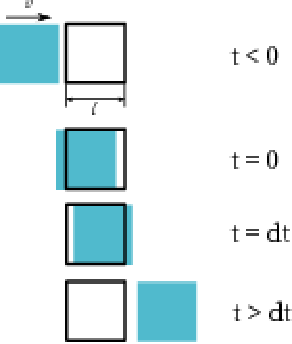
\includegraphics[width=0.45\textwidth]{images/resolution.pdf} 
		\caption{The control volumes in blue have the same size as the sensor (black rectangle). At $t=0$ the measurement starts and the first control volume is directly over the sensor. When  the measurement ends at $t=\tau$ the control volumes have moved. The sensor is covered by a mix of the two volumes.}
		\label{fig:cv}
	\end{center}
\end{figure}

To accommodate for that, factors $ n $ \eqref{eq:resn} and $ k $ \eqref{eq:resk} are introduced, describing the ratio of the resolutions to the actual sizes.

\begin{equation}
	n = \dfrac{l}{\diff s}
\label{eq:resn} 
\end{equation}

\begin{equation}
	k = \dfrac{ \tau}{\diff t}
\label{eq:resk}
\end{equation}

Inserting $ k $ and $ n $ in Equation \eqref{eq:resv} yields:

\begin{equation}
	v = \dfrac{\diff s}{\diff t} = \dfrac{k \cdot l}{n \cdot \tau}
\label{eq:resv1} 
\end{equation}

The ratio $ r $
\begin{equation}
	r = \frac{k}{n}
\label{eq:resr} 
\end{equation}
is the ratio of the time it takes a control volume to enter and leave the sensor area  to the time a measurement takes. Its inverse is the movement of the control volume during the measurement time and thereby the percentage by which the measured volume is bigger than the control volume. A ratio of 1 on would mean the measured volume is two times the sensor size, thereby halving the spacial resolution. To keep the resolution close the the sensor size, a ratio of 4, increasing the measured volume by \unit[25]{\%} is viable.
With the given sensor size and flow speed, a measurement time $ \tau $ of \unit[0.0025]{s} or \unit[2.5]{ms} is needed.\\

To test if the time resolution matches this, the measurement time itself can be timed. The difference between two adjacent times, i.e. the first time (\unit[975209221]{ns}) and the second time (\unit[975209961]{ns}), in the data set in Listing \ref{lst:data} is the measurement time of \unit[740]{ns}. The mean of the differences through the whole data set is \unit[748]{ns}. This means that the measurement is more than three times faster than required, showing that the time resolution easily matches the spacial resolution.

\begin{lstlisting}[caption={An excerpt of measurement data showing three lines of data from eight sensors. The long numbers are the times at which the measurements were taken in nanoseconds measured from the start, the short numbers are the measured values.},label={lst:data}]
975209221 21 975209961 59 975210676 15 975211397 0 975212119 0 975212840 26 975213554 59 975214276 9 
975215877 57 975216602 42 975217324 0 975218046 0 975218761 0 975219482 61 975220204 43 975220919 0 
975222520 52 975223271 0 975223993 0 975224708 0 975225429 45 975226150 53 975226867 0 975227583 0  
\end{lstlisting}

\subsection{Electrical Conductivity Resolution and Range}

Requirement: The system shall have a sensitivity of  \unit[0.1]{\%} salinity.\\
Requirement: The system shall have a range from 0 to \unit[5]{\%} salinity.\\

\subsection{Cost}

Requirement: The cost per sensor shall be less than \euro{25}\\

\subsection{Deployability in the Bioreactor}

Requirement: The system shall be deployable in the algae reactor.\\

The deployability was demonstrated during two test campaigns on the reactor. Figures \ref{fig:stripsr} and \ref{fig:pcr} show the set up during the tests. The host PC can be placed on a desk beside the reactor and connected to the carrier board with a USB cable. The carrier board can also be placed on desk or temporarily mounted on the reactor. The sensor strips connect to the carrier board with \unit[1]{m} long cables and are attached to the reactor with electrical tape.

\begin{figure}[H]
	\begin{center}
		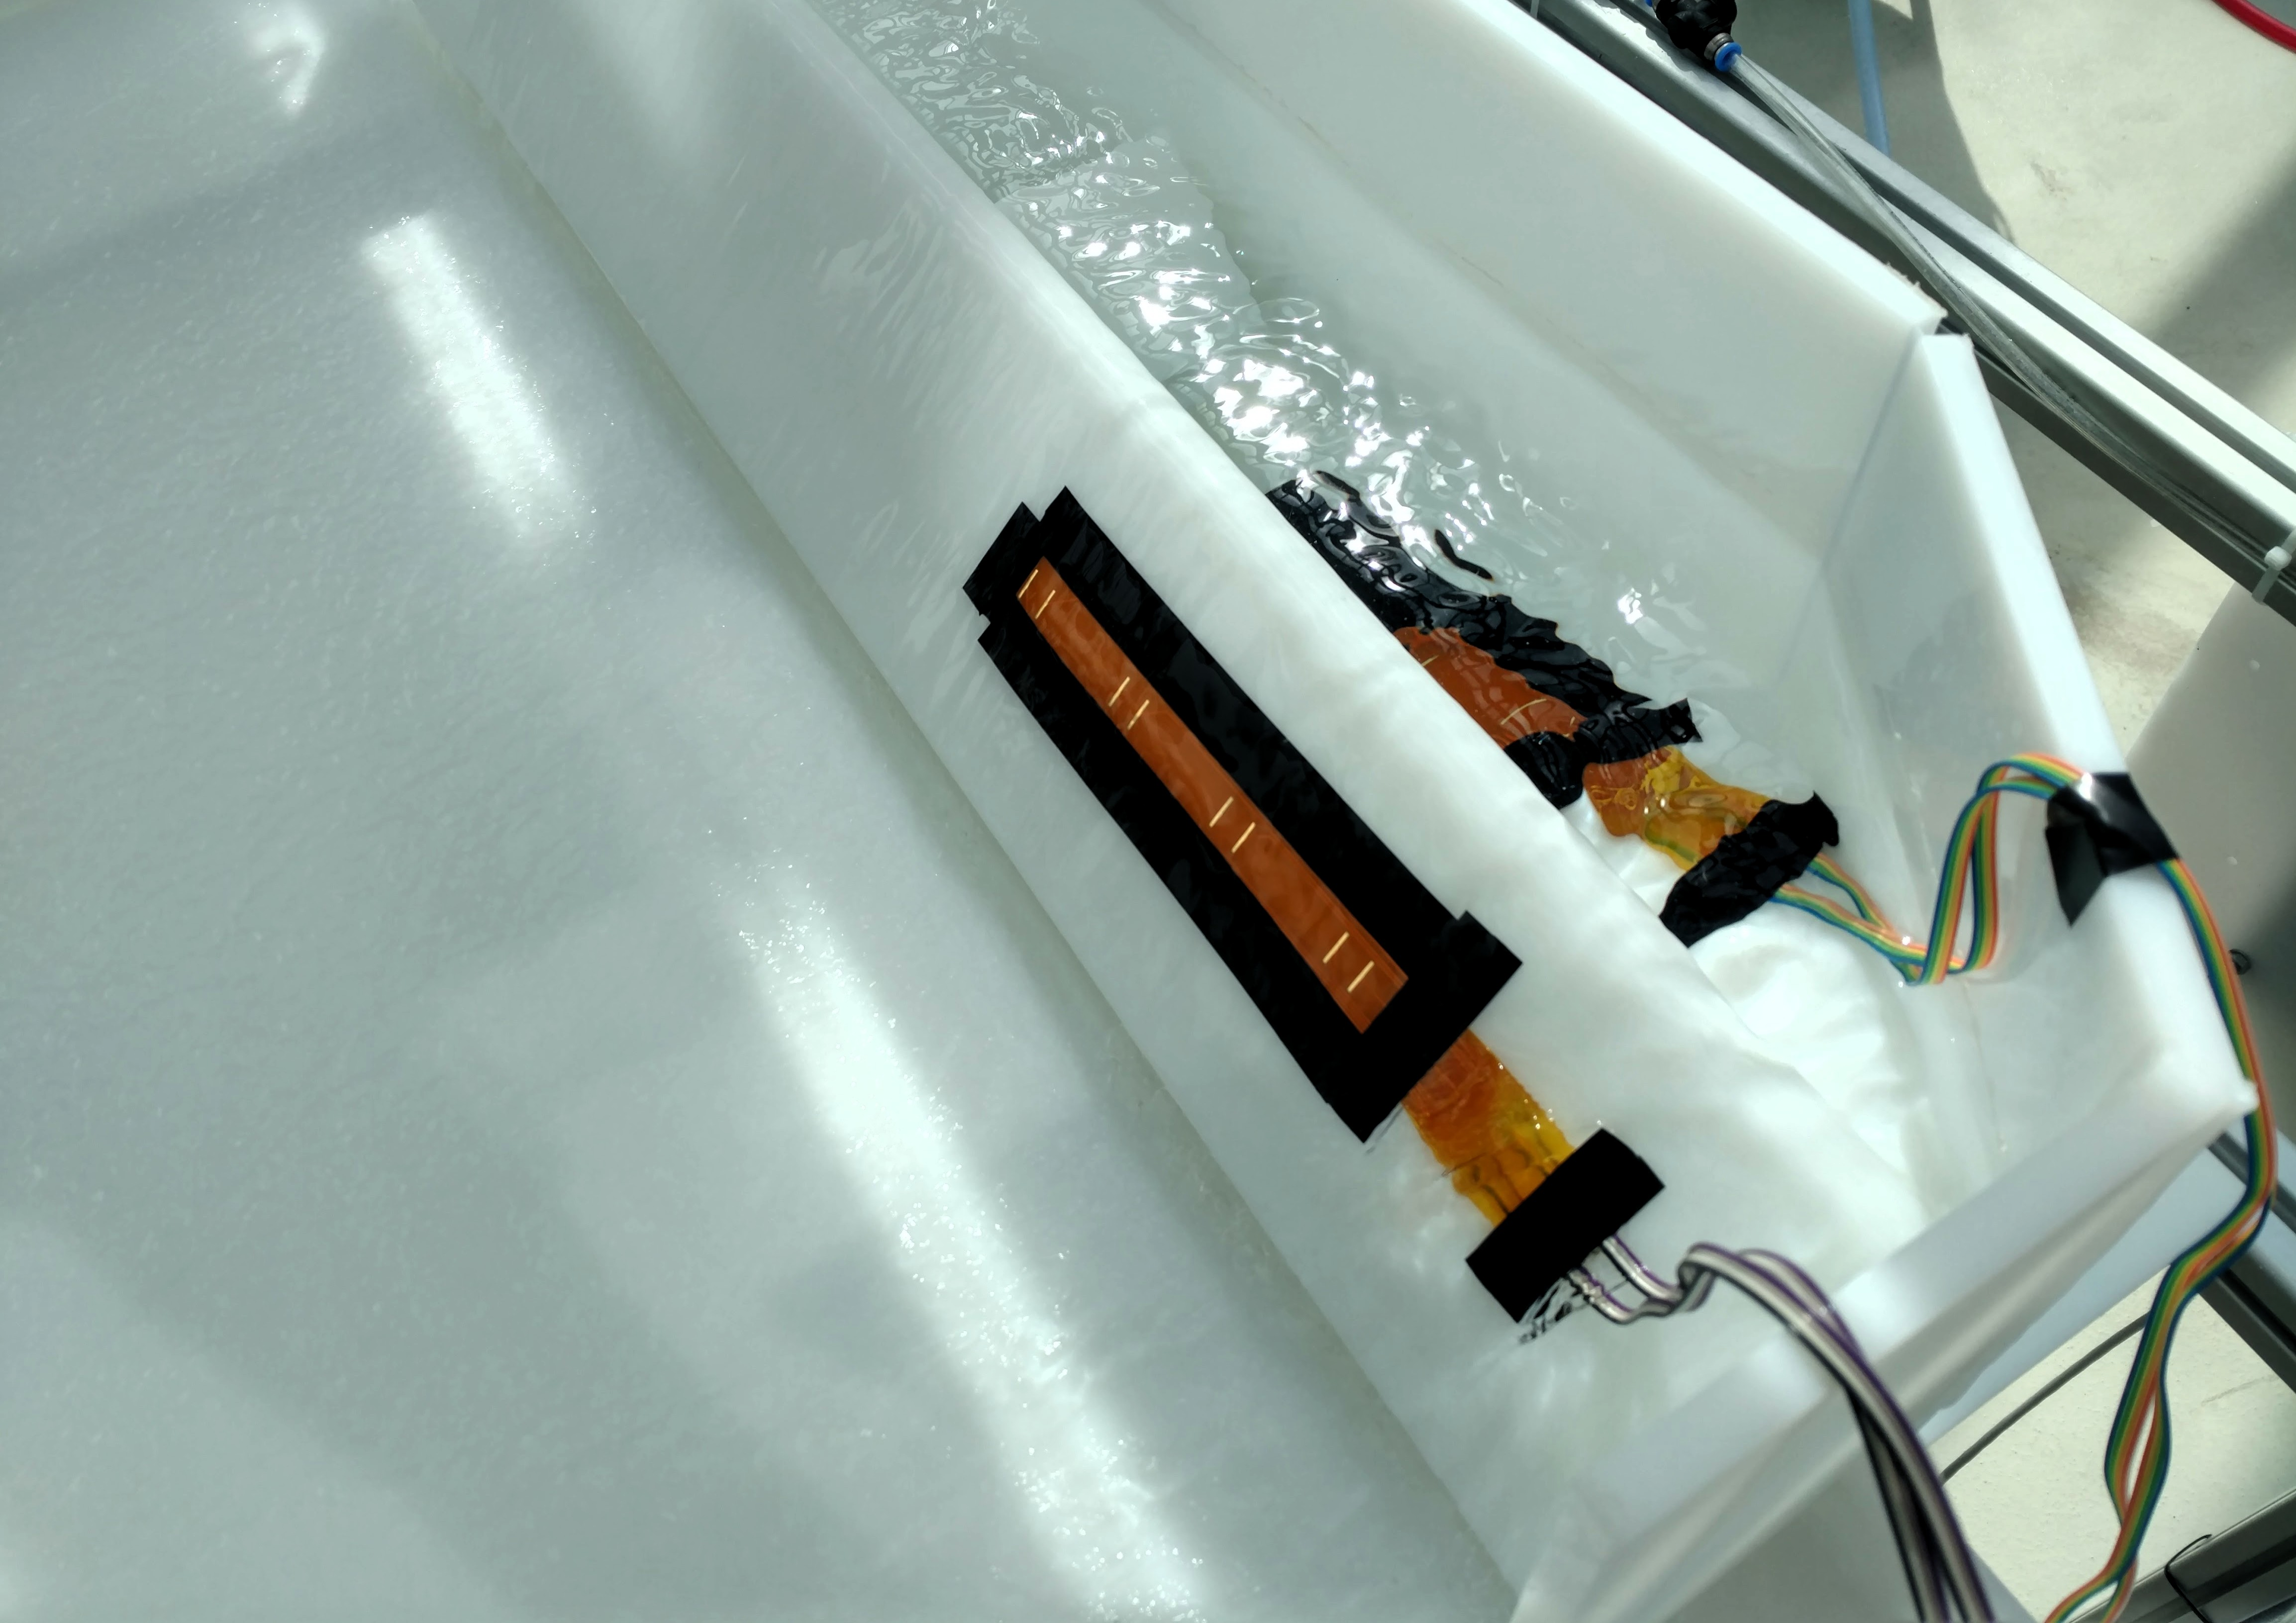
\includegraphics[width=0.8\textwidth]{images/stripsinreactor.jpg} 
		\caption{The sensor strips are mounted to the bioreactor with electrical tape. Cables of \unit[1]{m} length run towards the carrier board which is not in the frame.}
	\label{fig:stripsr}
	\end{center}
\end{figure}

\begin{figure}[H]
	\begin{center}
		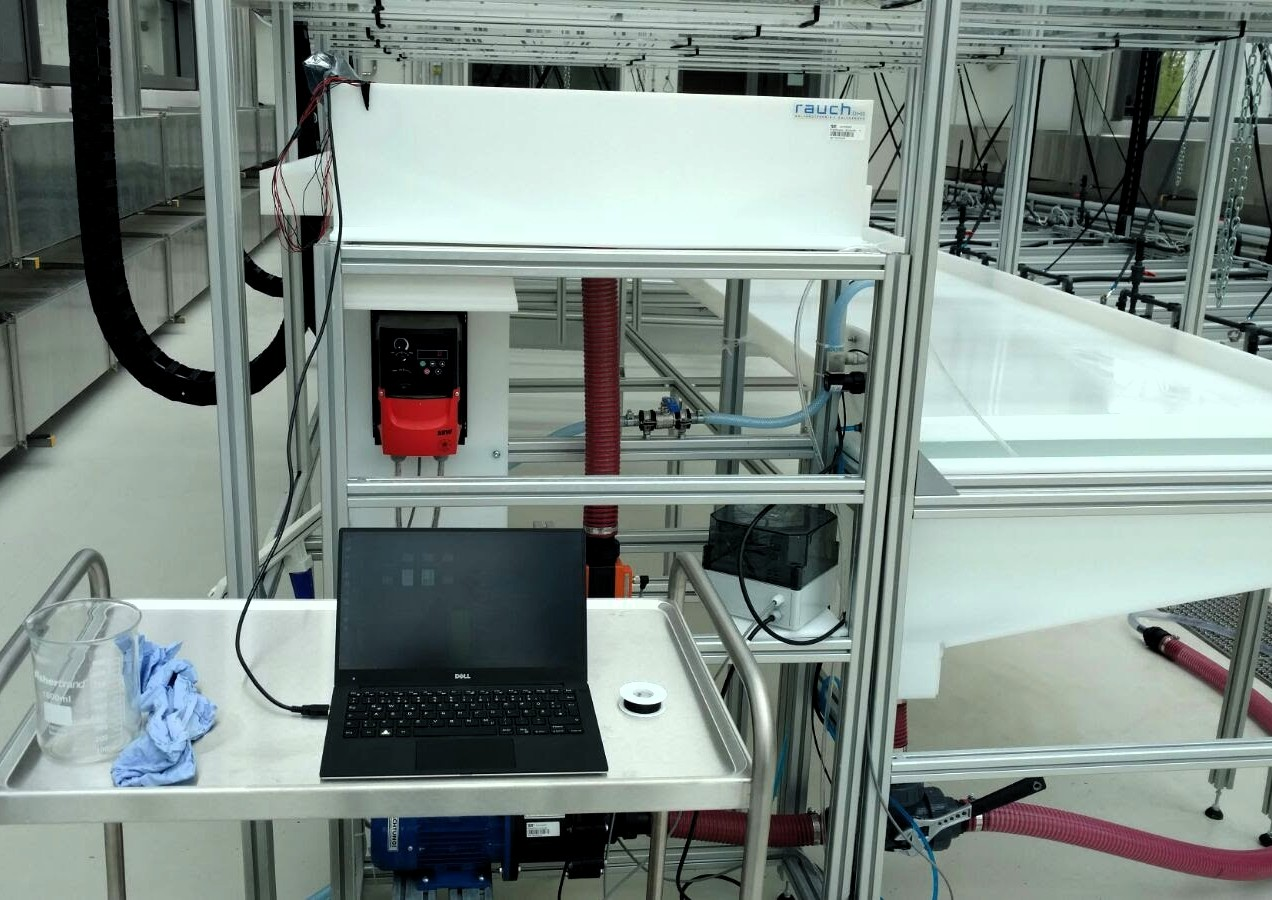
\includegraphics[width=0.8\textwidth]{images/pconreactor.jpg} 
		\caption{A laptop is used as host PC. A USB cable connects to the microcontroller on the carrier board, which is mounted on the side of the inlet basin.}
	\label{fig:pcr}
	\end{center}
\end{figure}

\subsection{Usability}

Requirement: The system shall be usable with a minimal set of written instructions.

\section{Validation}

\begin{figure}
	\begin{center}
		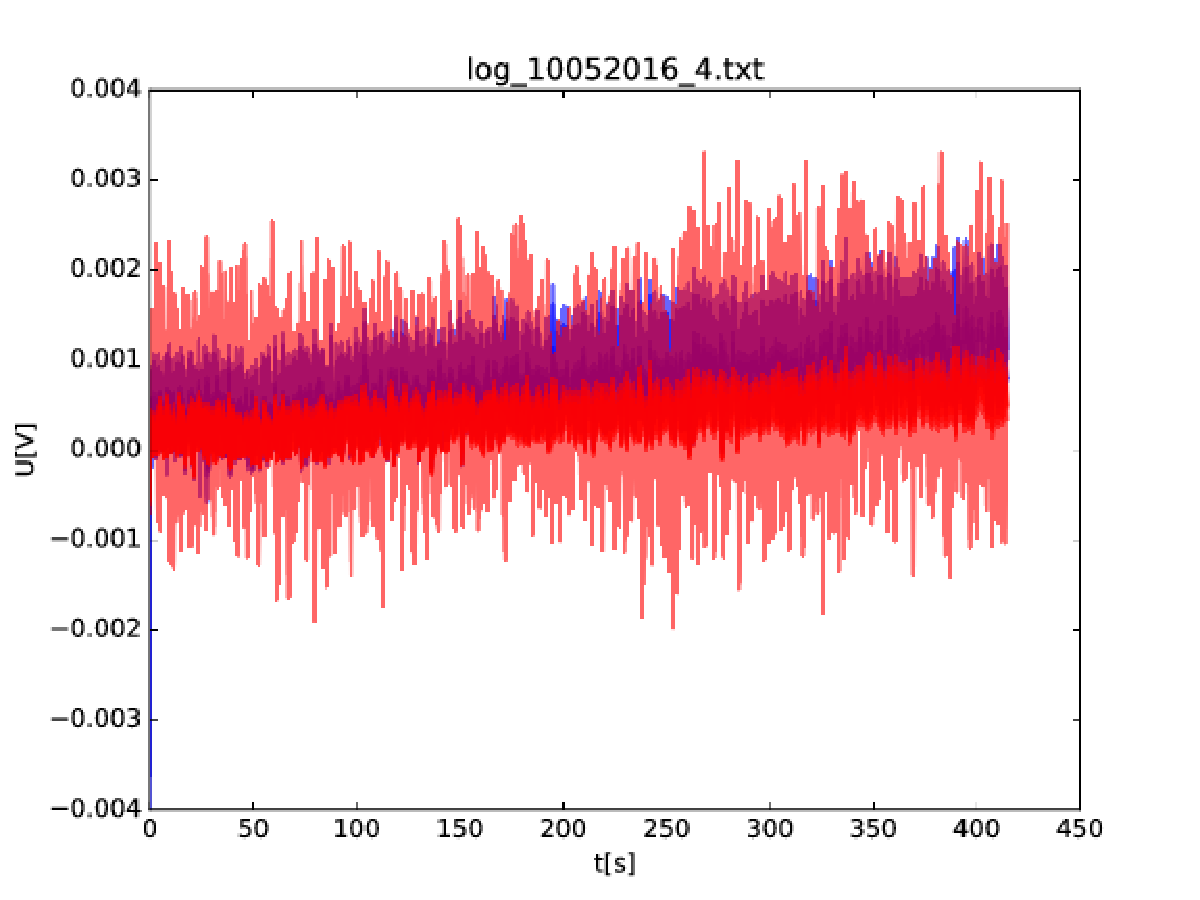
\includegraphics[width=\textwidth]{images/noise.pdf} 
		\caption{noise}
	\end{center}
\end{figure}

\begin{figure}
	\begin{center}
		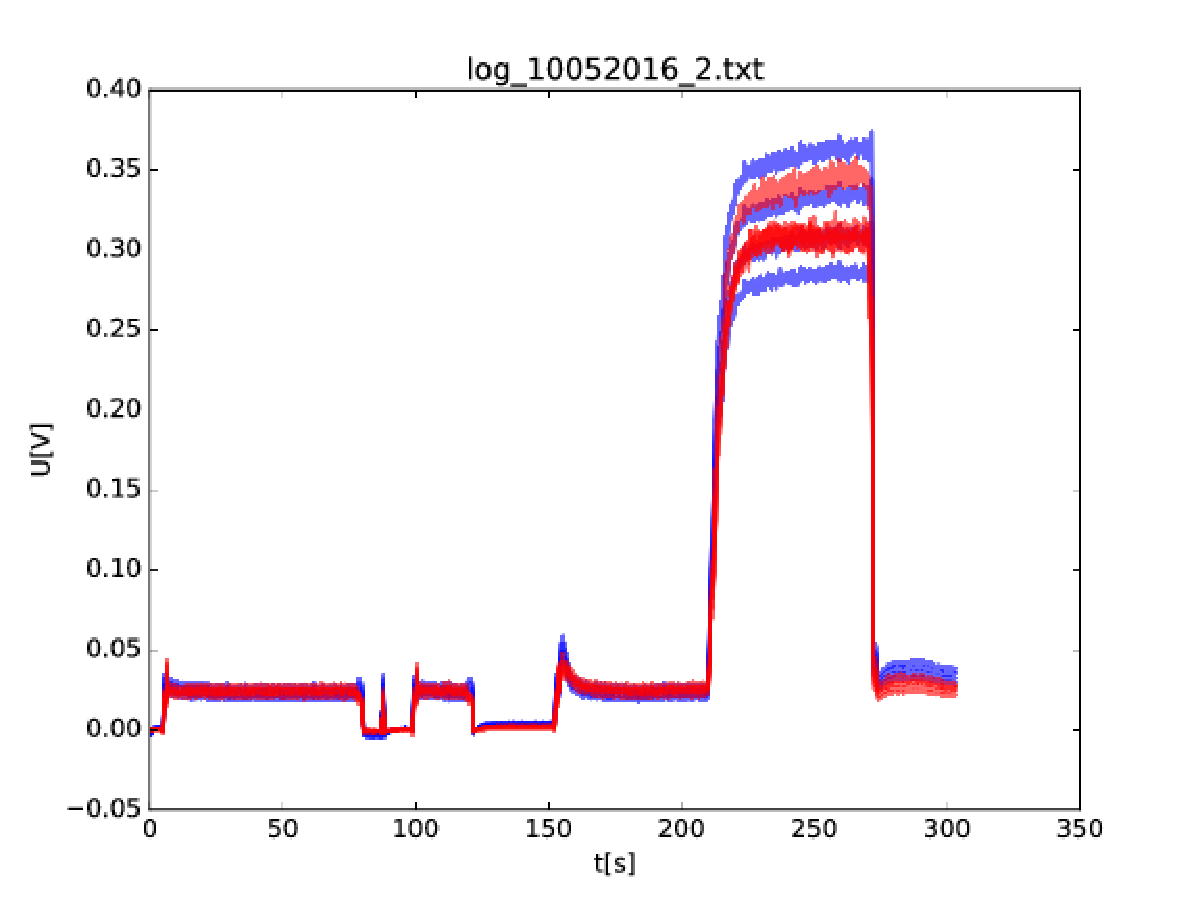
\includegraphics[width=\textwidth]{images/feed_switch.pdf} 
		\caption{feed switch}
	\end{center}
\end{figure}

\begin{figure}
	\begin{center}
		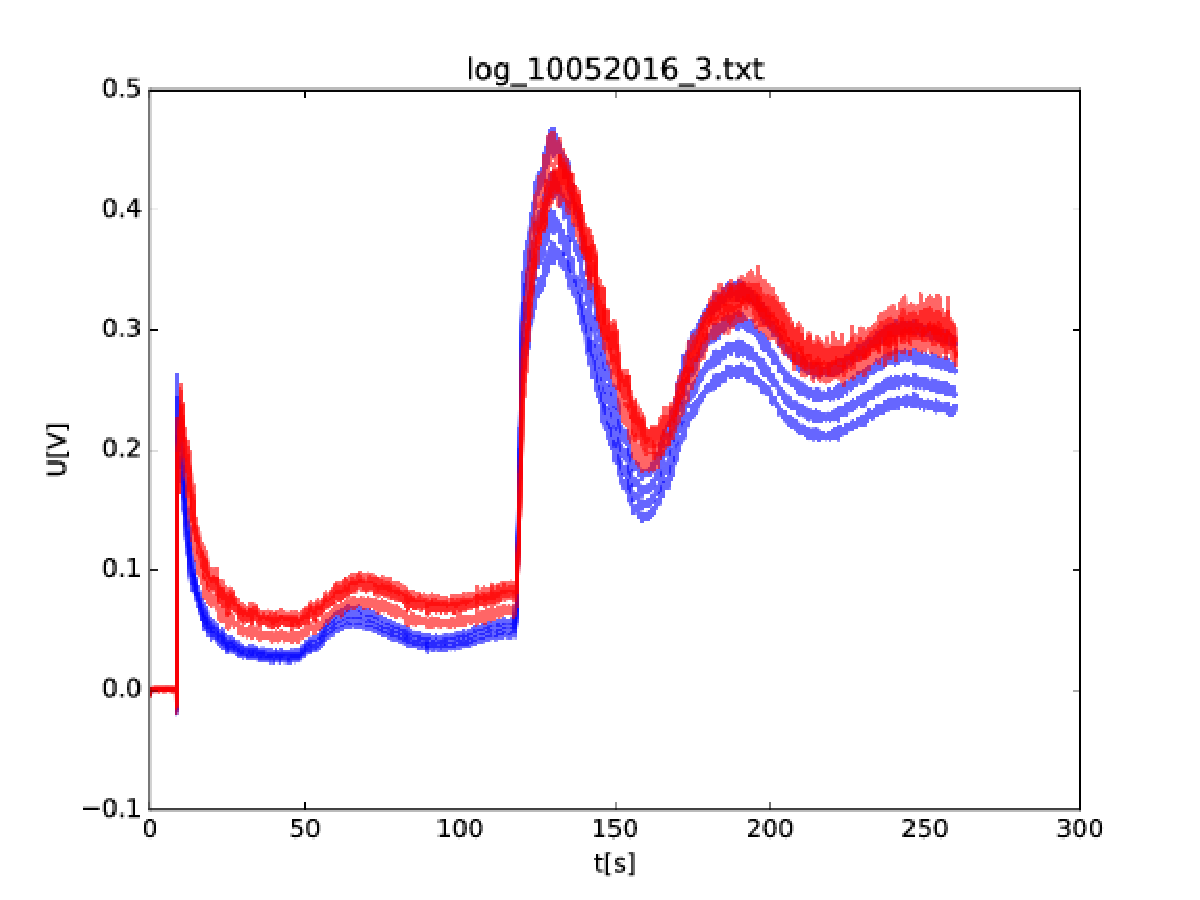
\includegraphics[width=\textwidth]{images/feed_add.pdf} 
		\caption{feed add}
	\end{center}
\end{figure}


